% Options for packages loaded elsewhere
% Options for packages loaded elsewhere
\PassOptionsToPackage{unicode}{hyperref}
\PassOptionsToPackage{hyphens}{url}
\PassOptionsToPackage{dvipsnames,svgnames,x11names}{xcolor}
%
\documentclass[
  letterpaper,
  DIV=11,
  numbers=noendperiod]{scrartcl}
\usepackage{xcolor}
\usepackage{amsmath,amssymb}
\setcounter{secnumdepth}{-\maxdimen} % remove section numbering
\usepackage{iftex}
\ifPDFTeX
  \usepackage[T1]{fontenc}
  \usepackage[utf8]{inputenc}
  \usepackage{textcomp} % provide euro and other symbols
\else % if luatex or xetex
  \usepackage{unicode-math} % this also loads fontspec
  \defaultfontfeatures{Scale=MatchLowercase}
  \defaultfontfeatures[\rmfamily]{Ligatures=TeX,Scale=1}
\fi
\usepackage{lmodern}
\ifPDFTeX\else
  % xetex/luatex font selection
\fi
% Use upquote if available, for straight quotes in verbatim environments
\IfFileExists{upquote.sty}{\usepackage{upquote}}{}
\IfFileExists{microtype.sty}{% use microtype if available
  \usepackage[]{microtype}
  \UseMicrotypeSet[protrusion]{basicmath} % disable protrusion for tt fonts
}{}
\makeatletter
\@ifundefined{KOMAClassName}{% if non-KOMA class
  \IfFileExists{parskip.sty}{%
    \usepackage{parskip}
  }{% else
    \setlength{\parindent}{0pt}
    \setlength{\parskip}{6pt plus 2pt minus 1pt}}
}{% if KOMA class
  \KOMAoptions{parskip=half}}
\makeatother
% Make \paragraph and \subparagraph free-standing
\makeatletter
\ifx\paragraph\undefined\else
  \let\oldparagraph\paragraph
  \renewcommand{\paragraph}{
    \@ifstar
      \xxxParagraphStar
      \xxxParagraphNoStar
  }
  \newcommand{\xxxParagraphStar}[1]{\oldparagraph*{#1}\mbox{}}
  \newcommand{\xxxParagraphNoStar}[1]{\oldparagraph{#1}\mbox{}}
\fi
\ifx\subparagraph\undefined\else
  \let\oldsubparagraph\subparagraph
  \renewcommand{\subparagraph}{
    \@ifstar
      \xxxSubParagraphStar
      \xxxSubParagraphNoStar
  }
  \newcommand{\xxxSubParagraphStar}[1]{\oldsubparagraph*{#1}\mbox{}}
  \newcommand{\xxxSubParagraphNoStar}[1]{\oldsubparagraph{#1}\mbox{}}
\fi
\makeatother

\usepackage{color}
\usepackage{fancyvrb}
\newcommand{\VerbBar}{|}
\newcommand{\VERB}{\Verb[commandchars=\\\{\}]}
\DefineVerbatimEnvironment{Highlighting}{Verbatim}{commandchars=\\\{\}}
% Add ',fontsize=\small' for more characters per line
\usepackage{framed}
\definecolor{shadecolor}{RGB}{241,243,245}
\newenvironment{Shaded}{\begin{snugshade}}{\end{snugshade}}
\newcommand{\AlertTok}[1]{\textcolor[rgb]{0.68,0.00,0.00}{#1}}
\newcommand{\AnnotationTok}[1]{\textcolor[rgb]{0.37,0.37,0.37}{#1}}
\newcommand{\AttributeTok}[1]{\textcolor[rgb]{0.40,0.45,0.13}{#1}}
\newcommand{\BaseNTok}[1]{\textcolor[rgb]{0.68,0.00,0.00}{#1}}
\newcommand{\BuiltInTok}[1]{\textcolor[rgb]{0.00,0.23,0.31}{#1}}
\newcommand{\CharTok}[1]{\textcolor[rgb]{0.13,0.47,0.30}{#1}}
\newcommand{\CommentTok}[1]{\textcolor[rgb]{0.37,0.37,0.37}{#1}}
\newcommand{\CommentVarTok}[1]{\textcolor[rgb]{0.37,0.37,0.37}{\textit{#1}}}
\newcommand{\ConstantTok}[1]{\textcolor[rgb]{0.56,0.35,0.01}{#1}}
\newcommand{\ControlFlowTok}[1]{\textcolor[rgb]{0.00,0.23,0.31}{\textbf{#1}}}
\newcommand{\DataTypeTok}[1]{\textcolor[rgb]{0.68,0.00,0.00}{#1}}
\newcommand{\DecValTok}[1]{\textcolor[rgb]{0.68,0.00,0.00}{#1}}
\newcommand{\DocumentationTok}[1]{\textcolor[rgb]{0.37,0.37,0.37}{\textit{#1}}}
\newcommand{\ErrorTok}[1]{\textcolor[rgb]{0.68,0.00,0.00}{#1}}
\newcommand{\ExtensionTok}[1]{\textcolor[rgb]{0.00,0.23,0.31}{#1}}
\newcommand{\FloatTok}[1]{\textcolor[rgb]{0.68,0.00,0.00}{#1}}
\newcommand{\FunctionTok}[1]{\textcolor[rgb]{0.28,0.35,0.67}{#1}}
\newcommand{\ImportTok}[1]{\textcolor[rgb]{0.00,0.46,0.62}{#1}}
\newcommand{\InformationTok}[1]{\textcolor[rgb]{0.37,0.37,0.37}{#1}}
\newcommand{\KeywordTok}[1]{\textcolor[rgb]{0.00,0.23,0.31}{\textbf{#1}}}
\newcommand{\NormalTok}[1]{\textcolor[rgb]{0.00,0.23,0.31}{#1}}
\newcommand{\OperatorTok}[1]{\textcolor[rgb]{0.37,0.37,0.37}{#1}}
\newcommand{\OtherTok}[1]{\textcolor[rgb]{0.00,0.23,0.31}{#1}}
\newcommand{\PreprocessorTok}[1]{\textcolor[rgb]{0.68,0.00,0.00}{#1}}
\newcommand{\RegionMarkerTok}[1]{\textcolor[rgb]{0.00,0.23,0.31}{#1}}
\newcommand{\SpecialCharTok}[1]{\textcolor[rgb]{0.37,0.37,0.37}{#1}}
\newcommand{\SpecialStringTok}[1]{\textcolor[rgb]{0.13,0.47,0.30}{#1}}
\newcommand{\StringTok}[1]{\textcolor[rgb]{0.13,0.47,0.30}{#1}}
\newcommand{\VariableTok}[1]{\textcolor[rgb]{0.07,0.07,0.07}{#1}}
\newcommand{\VerbatimStringTok}[1]{\textcolor[rgb]{0.13,0.47,0.30}{#1}}
\newcommand{\WarningTok}[1]{\textcolor[rgb]{0.37,0.37,0.37}{\textit{#1}}}

\usepackage{longtable,booktabs,array}
\usepackage{calc} % for calculating minipage widths
% Correct order of tables after \paragraph or \subparagraph
\usepackage{etoolbox}
\makeatletter
\patchcmd\longtable{\par}{\if@noskipsec\mbox{}\fi\par}{}{}
\makeatother
% Allow footnotes in longtable head/foot
\IfFileExists{footnotehyper.sty}{\usepackage{footnotehyper}}{\usepackage{footnote}}
\makesavenoteenv{longtable}
\usepackage{graphicx}
\makeatletter
\newsavebox\pandoc@box
\newcommand*\pandocbounded[1]{% scales image to fit in text height/width
  \sbox\pandoc@box{#1}%
  \Gscale@div\@tempa{\textheight}{\dimexpr\ht\pandoc@box+\dp\pandoc@box\relax}%
  \Gscale@div\@tempb{\linewidth}{\wd\pandoc@box}%
  \ifdim\@tempb\p@<\@tempa\p@\let\@tempa\@tempb\fi% select the smaller of both
  \ifdim\@tempa\p@<\p@\scalebox{\@tempa}{\usebox\pandoc@box}%
  \else\usebox{\pandoc@box}%
  \fi%
}
% Set default figure placement to htbp
\def\fps@figure{htbp}
\makeatother





\setlength{\emergencystretch}{3em} % prevent overfull lines

\providecommand{\tightlist}{%
  \setlength{\itemsep}{0pt}\setlength{\parskip}{0pt}}



 


\KOMAoption{captions}{tableheading}
\makeatletter
\@ifpackageloaded{caption}{}{\usepackage{caption}}
\AtBeginDocument{%
\ifdefined\contentsname
  \renewcommand*\contentsname{Table of contents}
\else
  \newcommand\contentsname{Table of contents}
\fi
\ifdefined\listfigurename
  \renewcommand*\listfigurename{List of Figures}
\else
  \newcommand\listfigurename{List of Figures}
\fi
\ifdefined\listtablename
  \renewcommand*\listtablename{List of Tables}
\else
  \newcommand\listtablename{List of Tables}
\fi
\ifdefined\figurename
  \renewcommand*\figurename{Figure}
\else
  \newcommand\figurename{Figure}
\fi
\ifdefined\tablename
  \renewcommand*\tablename{Table}
\else
  \newcommand\tablename{Table}
\fi
}
\@ifpackageloaded{float}{}{\usepackage{float}}
\floatstyle{ruled}
\@ifundefined{c@chapter}{\newfloat{codelisting}{h}{lop}}{\newfloat{codelisting}{h}{lop}[chapter]}
\floatname{codelisting}{Listing}
\newcommand*\listoflistings{\listof{codelisting}{List of Listings}}
\makeatother
\makeatletter
\makeatother
\makeatletter
\@ifpackageloaded{caption}{}{\usepackage{caption}}
\@ifpackageloaded{subcaption}{}{\usepackage{subcaption}}
\makeatother
\usepackage{bookmark}
\IfFileExists{xurl.sty}{\usepackage{xurl}}{} % add URL line breaks if available
\urlstyle{same}
\hypersetup{
  pdftitle={💬  🤖 Asking questions to your database with LLMs},
  pdfauthor={Nahuel Defossé  nahuel.defosse@ibm.com IBM Research Africa},
  colorlinks=true,
  linkcolor={blue},
  filecolor={Maroon},
  citecolor={Blue},
  urlcolor={Blue},
  pdfcreator={LaTeX via pandoc}}


\title{💬 🤖 Asking questions to your database with LLMs}
\author{Nahuel Defossé
\href{mailto:nahuel.defosse@ibm.com}{\nolinkurl{nahuel.defosse@ibm.com}}IBM
Research Africa}
\date{}
\begin{document}
\maketitle


\begin{Shaded}
\begin{Highlighting}[]
\ImportTok{import}\NormalTok{ os}
\NormalTok{os.environ[}\StringTok{"JUPYTER\_COLUMNS"}\NormalTok{] }\OperatorTok{=} \StringTok{"60"}
\CommentTok{\# \%load\_ext rich}
\end{Highlighting}
\end{Shaded}

\subsection{About myself}\label{about-myself}


\includegraphics[width=\linewidth,height=12em,keepaspectratio]{./img/memes/myself.gif}

\begin{itemize}
\tightlist
\item
  🐍 Pythonista with 18 years of experience.

  \begin{itemize}
  \tightlist
  \item
    Co-organized SciPy Latin America
  \end{itemize}
\item
  🚜 Worked as CTO in Hello Tractor
\item
  🧪 Software Engineer at IBM Research
\item
  🛰️ Worked in Foundational Models for Geospatial applications

  \begin{itemize}
  \tightlist
  \item
    \href{https://pycon-kenya-2025.sessionize.com/session/954933}{There's
    a workshop on Saturday 🤩}
  \end{itemize}
\item
  💬 Currently working on
  \href{https://research.ibm.com/projects/flowpilot}{Flowpilot },
  providing core features to different products and divisions.
\end{itemize}

\begin{center}\rule{0.5\linewidth}{0.5pt}\end{center}

\begin{center}\rule{0.5\linewidth}{0.5pt}\end{center}

\section{Intro}\label{intro}

In this talk we're gonna show how to use Python to:

\begin{itemize}
\tightlist
\item
  Connect to a database and execute the queries (🐦)
\item
  Convert natural language questions into SQL
\item
  Create a workflow
\item
  More advanced nodes
\item
  Lessons learned
\end{itemize}

TODO: Put some drawing \& rephrase

\begin{center}\rule{0.5\linewidth}{0.5pt}\end{center}

\section{Connect to a database and execute the
queries}\label{connect-to-a-database-and-execute-the-queries}

\begin{center}\rule{0.5\linewidth}{0.5pt}\end{center}

\subsection{Public datasets used in text to
SQL}\label{public-datasets-used-in-text-to-sql}

These datasets define:

\begin{itemize}
\tightlist
\item
  ❓ Natural language questions
\item
  🫰 Expected SQL
\item
  🏗️ Database schema \& content
\item
  🔎 Evaluation metrics
\item
  🥇 Leaderboard
\end{itemize}

\begin{itemize}
\tightlist
\item
  \href{https://yale-lily.github.io/spider}{🕷️ Spider}
\end{itemize}

\begin{itemize}
\tightlist
\item
  \href{https://spider2-sql.github.io/}{🕷️ 🕷️ Spider 2}
\end{itemize}

\begin{itemize}
\tightlist
\item
  🐦 \href{https://bird-bench.github.io/}{BIRD}
\end{itemize}

\begin{itemize}
\tightlist
\item
  \href{https://sig4kg.github.io/archer-bench/}{🏹 Archer}
\end{itemize}

\begin{center}\rule{0.5\linewidth}{0.5pt}\end{center}

\subsection{BIRD}\label{bird}

\begin{figure}[H]

{\centering 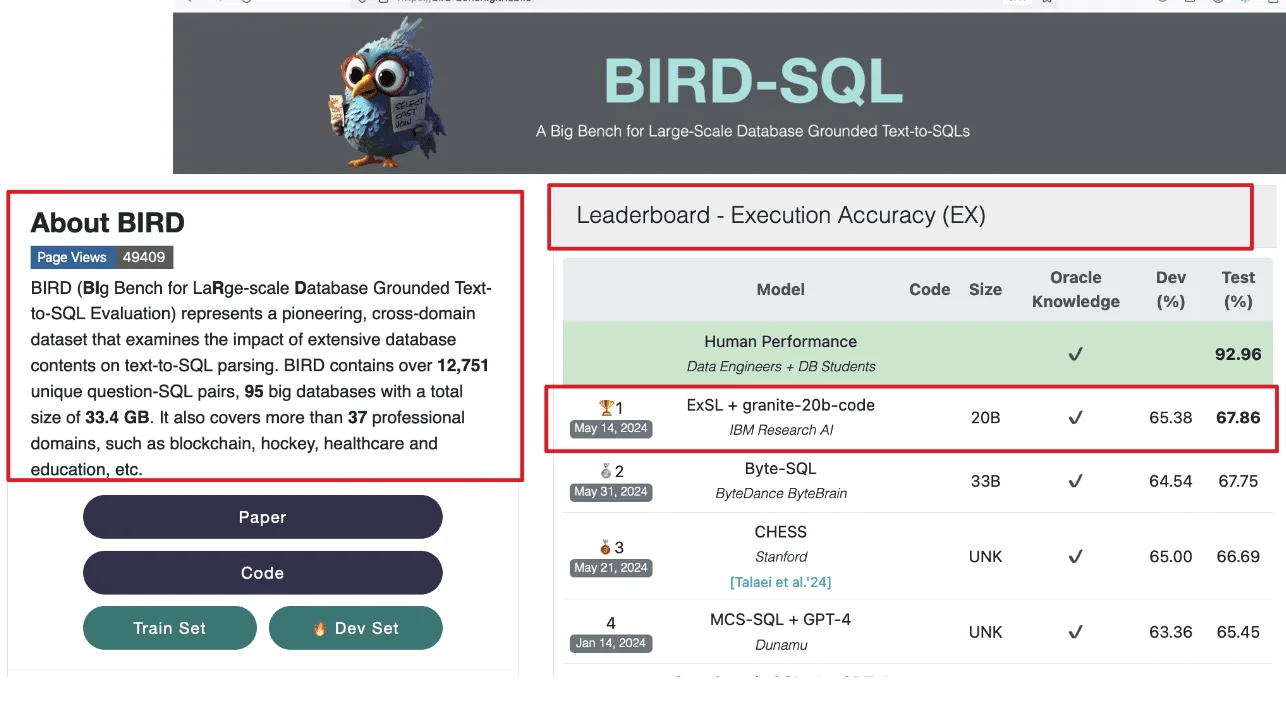
\includegraphics[width=\linewidth,height=4.16667in,keepaspectratio]{./img/ibm-granite-leaderboard.png}

}

\caption{\href{https://research.ibm.com/blog/granite-LLM-text-to-SQL}{IBM
Research in the lederboard 2024-06-02}}

\end{figure}%

We're select BIRD dataset since we have some experience with it, we
managed to get to the top of the leatherboard in 2024/6

\begin{center}\rule{0.5\linewidth}{0.5pt}\end{center}

\subsubsection{BIRD mini-dev}\label{bird-mini-dev}

\begin{itemize}
\tightlist
\item
  It consist of 500 queries classified as \textbf{simple},
  \textbf{moderate} and \textbf{challenging}
  \href{https://github.com/bird-bench/mini_dev}{}
\end{itemize}

\begin{Shaded}
\begin{Highlighting}[]
\ImportTok{from}\NormalTok{ rich.console }\ImportTok{import}\NormalTok{ Console}
\NormalTok{\_c }\OperatorTok{=}\NormalTok{ Console(width}\OperatorTok{=}\DecValTok{45}\NormalTok{)}
\CommentTok{\# Ensure print are contained within the range}
\BuiltInTok{print} \OperatorTok{=}\NormalTok{ \_c.}\BuiltInTok{print}


\ImportTok{from}\NormalTok{ IPython.display }\ImportTok{import}\NormalTok{ display, Image}
\end{Highlighting}
\end{Shaded}

\begin{Shaded}
\begin{Highlighting}[]
\ImportTok{from}\NormalTok{ datasets }\ImportTok{import}\NormalTok{ load\_dataset, DownloadConfig }

\CommentTok{\# Load the dataset}
\NormalTok{dataset }\OperatorTok{=}\NormalTok{ load\_dataset(}
  \StringTok{"birdsql/bird\_mini\_dev"}\NormalTok{, }
\NormalTok{  download\_config}\OperatorTok{=}\NormalTok{DownloadConfig(disable\_tqdm}\OperatorTok{=}\VariableTok{True}\NormalTok{)}
\NormalTok{)}

\CommentTok{\# Contents}
\BuiltInTok{print}\NormalTok{(}\StringTok{"Database types: "}\NormalTok{, }\OperatorTok{*}\NormalTok{dataset.keys())}
\NormalTok{sqlite\_df }\OperatorTok{=}\NormalTok{ dataset[}\StringTok{"mini\_dev\_sqlite"}\NormalTok{].to\_pandas()}
\NormalTok{sqlite\_df }\OperatorTok{=}\NormalTok{ sqlite\_df.drop(columns}\OperatorTok{=}\NormalTok{[}\StringTok{\textquotesingle{}question\_id\textquotesingle{}}\NormalTok{])}
\NormalTok{display(sqlite\_df.head(}\DecValTok{5}\NormalTok{))}
\end{Highlighting}
\end{Shaded}

\begin{verbatim}
Database types:  mini_dev_mysql mini_dev_pg 
mini_dev_sqlite
\end{verbatim}

\begin{longtable}[]{@{}llllll@{}}
\toprule\noalign{}
& db\_id & question & evidence & SQL & difficulty \\
\midrule\noalign{}
\endhead
\bottomrule\noalign{}
\endlastfoot
0 & debit\_card\_specializing & What is the ratio of customers who pay
in EUR ... & ratio of customers who pay in EUR against cust... & SELECT
CAST(SUM(IIF(Currency = \textquotesingle EUR\textquotesingle, 1, 0))
A... & simple \\
1 & debit\_card\_specializing & In 2012, who had the least consumption
in LAM? & Year 2012 can be presented as Between 201201 A... & SELECT
T1.CustomerID FROM customers AS T1 INNE... & moderate \\
2 & debit\_card\_specializing & What was the average monthly consumption
of cu... & Average Monthly consumption = AVG(Consumption)... & SELECT
AVG(T2.Consumption) / 12 FROM customers... & moderate \\
3 & debit\_card\_specializing & What was the difference in gas
consumption bet... & Year 2012 can be presented as Between 201201 A... &
SELECT SUM(IIF(T1.Currency = \textquotesingle CZK\textquotesingle,
T2.Consump... & challenging \\
4 & debit\_card\_specializing & Which year recorded the most consumption
of ga... & The first 4 strings of the Date values in the ... & SELECT
SUBSTR(T2.Date, 1, 4) FROM customers AS... & moderate \\
\end{longtable}

\begin{center}\rule{0.5\linewidth}{0.5pt}\end{center}

\subsubsection{Downloading BIRD
databases}\label{downloading-bird-databases}

\begin{Shaded}
\begin{Highlighting}[]
\NormalTok{uvx gdown https://drive.google.com/file/d/13VLWIwpw5E3d5DUkMvzw7hvHE67a4XkG/}
\end{Highlighting}
\end{Shaded}

\pandocbounded{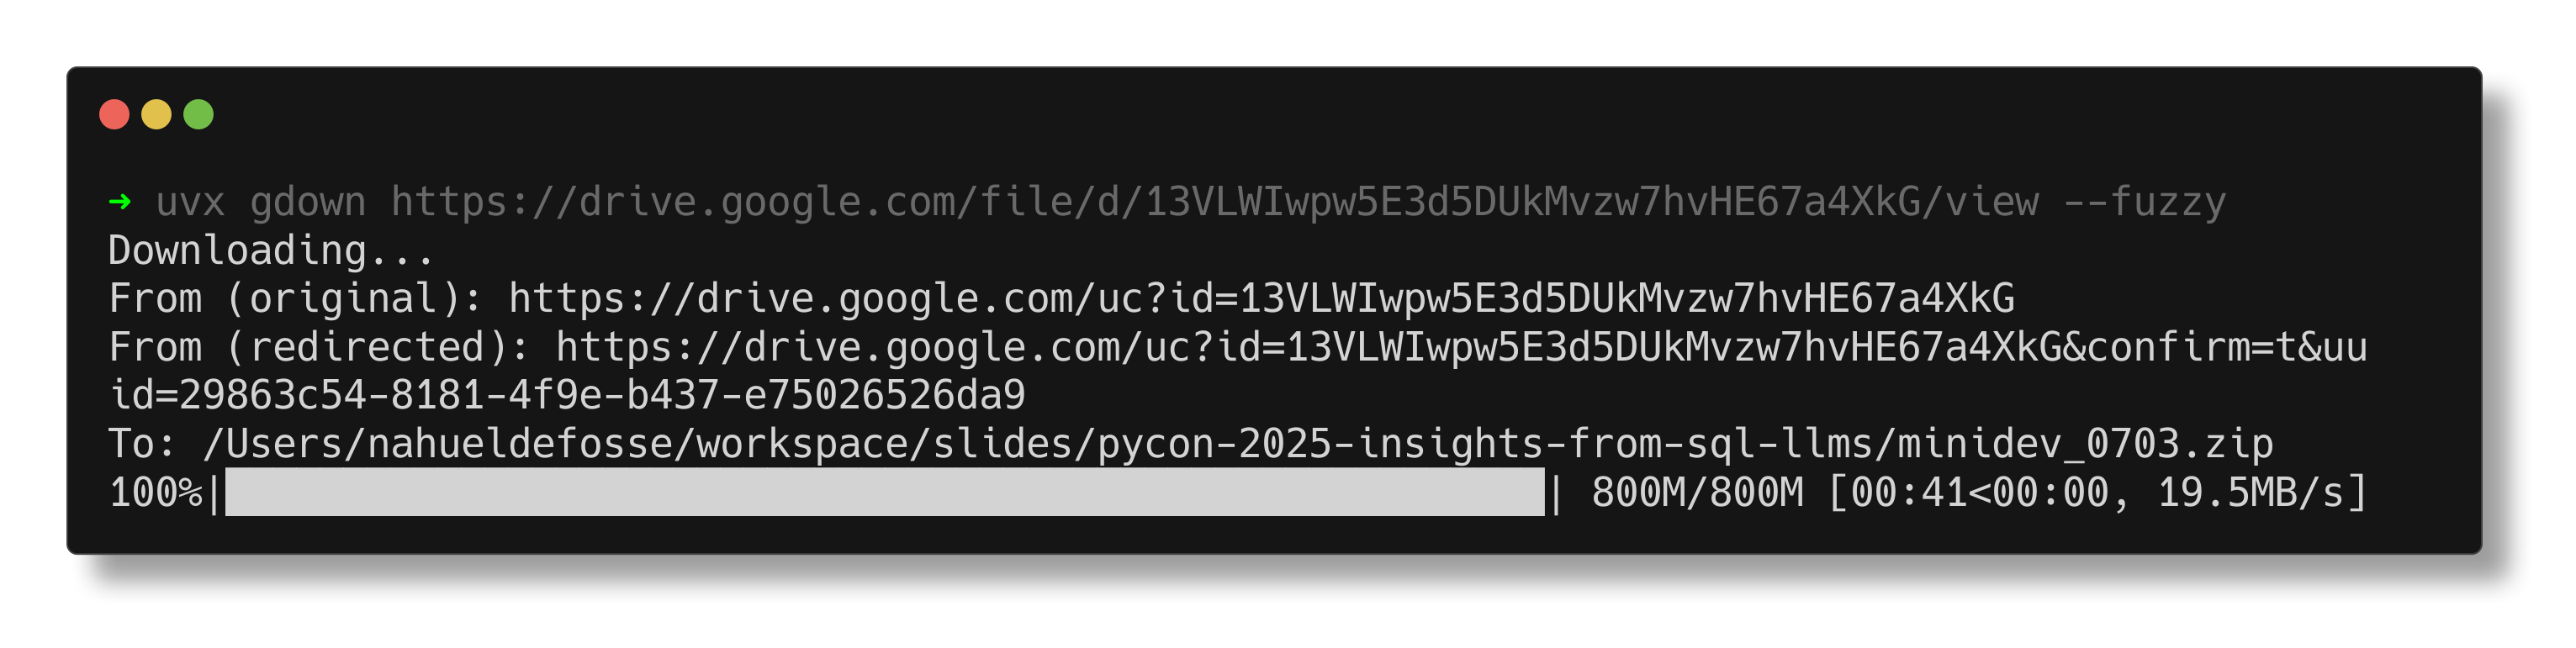
\includegraphics[keepaspectratio]{./img/download_minidev.png}}

Extracting the archive (3.3GiB)

\begin{Shaded}
\begin{Highlighting}[]
\NormalTok{unzip minidev\_703.zip}
\end{Highlighting}
\end{Shaded}

\begin{center}\rule{0.5\linewidth}{0.5pt}\end{center}

\subsubsection{\texorpdfstring{Picking the example database
\texttt{california\_schools}}{Picking the example database california\_schools}}\label{picking-the-example-database-california_schools}

In \texttt{minidev/MINIDEV/dev\_databases/california\_schools/} we find
the

\pandocbounded{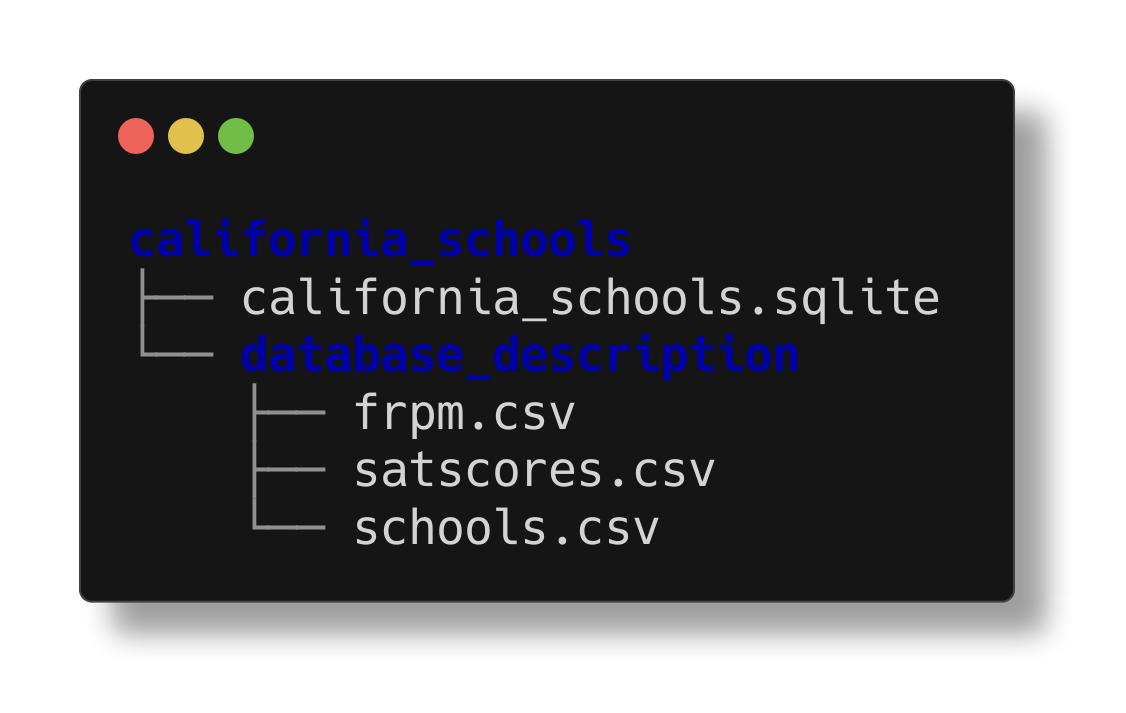
\includegraphics[keepaspectratio]{./img/california_school.png}}

\begin{Shaded}
\begin{Highlighting}[]
\ImportTok{from}\NormalTok{ pathlib }\ImportTok{import}\NormalTok{ Path}
\NormalTok{base }\OperatorTok{=}\NormalTok{ Path(}\StringTok{\textquotesingle{}./minidev/MINIDEV/dev\_databases/california\_schools/\textquotesingle{}}\NormalTok{)}
\end{Highlighting}
\end{Shaded}

\begin{center}\rule{0.5\linewidth}{0.5pt}\end{center}

\subsubsection{\texorpdfstring{Creating the
\texttt{Engine}}{Creating the Engine}}\label{creating-the-engine}

Creating an \texttt{Engine} instance connected to a SQLite database.

\begin{Shaded}
\begin{Highlighting}[]
\ImportTok{from}\NormalTok{ sqlalchemy }\ImportTok{import}\NormalTok{ create\_engine}
\NormalTok{db\_path }\OperatorTok{=}\NormalTok{ base }\OperatorTok{/} \StringTok{\textquotesingle{}california\_schools.sqlite\textquotesingle{}}
\NormalTok{db\_url }\OperatorTok{=} \SpecialStringTok{f"sqlite:///}\SpecialCharTok{\{}\NormalTok{db\_path}\SpecialCharTok{\}}\SpecialStringTok{"}
\NormalTok{engine }\OperatorTok{=}\NormalTok{ create\_engine(db\_url)}
\NormalTok{engine}
\end{Highlighting}
\end{Shaded}

\begin{verbatim}
Engine(sqlite:///minidev/MINIDEV/dev_databases/california_schools/california_schools.sqlite)
\end{verbatim}

\begin{center}\rule{0.5\linewidth}{0.5pt}\end{center}

\subsection{ER}\label{er}

\begin{Shaded}
\begin{Highlighting}[]
\CommentTok{\#from eralchemy import render\_er}
\CommentTok{\#render\_er(db\_url, \textquotesingle{}./img/output/erd\_from\_sqlite.svg\textquotesingle{})}
\end{Highlighting}
\end{Shaded}

\pandocbounded{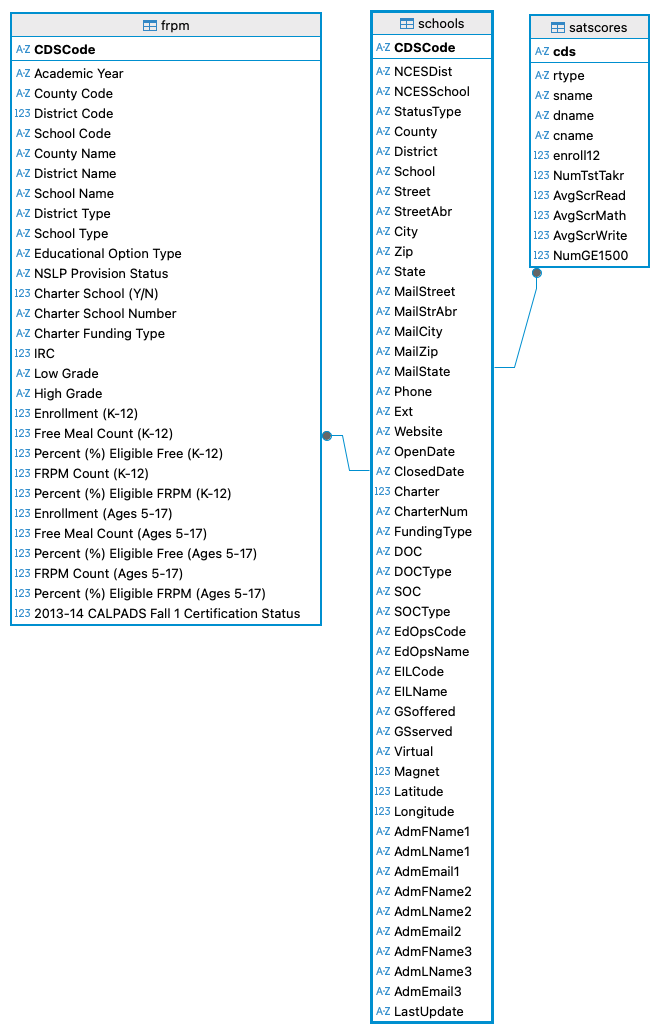
\includegraphics[keepaspectratio]{./img/er-california-schools.png}}

\begin{center}\rule{0.5\linewidth}{0.5pt}\end{center}

\subsubsection{Getting one simple
question}\label{getting-one-simple-question}

\begin{Shaded}
\begin{Highlighting}[]
\NormalTok{simple\_queries\_df }\OperatorTok{=}\NormalTok{ (sqlite\_df}
\NormalTok{  .pipe(}\KeywordTok{lambda}\NormalTok{ df: df[df.db\_id }\OperatorTok{==} \StringTok{\textquotesingle{}california\_schools\textquotesingle{}}\NormalTok{])}
\NormalTok{  .pipe(}\KeywordTok{lambda}\NormalTok{ df: df[df.difficulty }\OperatorTok{==} \StringTok{\textquotesingle{}simple\textquotesingle{}}\NormalTok{]))}

\NormalTok{simple\_queries\_df.head(}\DecValTok{2}\NormalTok{).set\_index(}\StringTok{"db\_id"}\NormalTok{)}
\end{Highlighting}
\end{Shaded}

\begin{longtable}[]{@{}lllll@{}}
\toprule\noalign{}
& question & evidence & SQL & difficulty \\
db\_id & & & & \\
\midrule\noalign{}
\endhead
\bottomrule\noalign{}
\endlastfoot
california\_schools & How many schools with an average score in Math...
& Exclusively virtual refers to Virtual =
\textquotesingle F\textquotesingle{} & SELECT COUNT(DISTINCT T2.School)
FROM satscore... & simple \\
california\_schools & Please list the codes of the schools with a to...
& Total enrollment can be represented by `Enroll... & SELECT T2.CDSCode
FROM schools AS T1 INNER JOI... & simple \\
\end{longtable}

\begin{center}\rule{0.5\linewidth}{0.5pt}\end{center}

\subsubsection{Getting one simple
question}\label{getting-one-simple-question-1}

\begin{Shaded}
\begin{Highlighting}[]
\NormalTok{question\_sql\_df }\OperatorTok{=}\NormalTok{ (simple\_queries\_df}
\NormalTok{  .pipe(}\KeywordTok{lambda}\NormalTok{ df: df[[}\StringTok{"question"}\NormalTok{, }\StringTok{"SQL"}\NormalTok{]])}
\NormalTok{  .reset\_index())}
\end{Highlighting}
\end{Shaded}

Let's take a look at the \texttt{question} and \texttt{SQL} column.

\begin{Shaded}
\begin{Highlighting}[]
\NormalTok{question, query }\OperatorTok{=}\NormalTok{ question\_sql\_df.loc[}
  \DecValTok{0}\NormalTok{, }
\NormalTok{  [}\StringTok{"question"}\NormalTok{, }\StringTok{"SQL"}\NormalTok{]]}
\NormalTok{display(question, query)}
\end{Highlighting}
\end{Shaded}

\begin{verbatim}
'How many schools with an average score in Math greater than 400 in the SAT test are exclusively virtual?'
\end{verbatim}

\begin{verbatim}
"SELECT COUNT(DISTINCT T2.School) FROM satscores AS T1 INNER JOIN schools AS T2 ON T1.cds = T2.CDSCode WHERE T2.Virtual = 'F' AND T1.AvgScrMath > 400"
\end{verbatim}

\begin{center}\rule{0.5\linewidth}{0.5pt}\end{center}

\subsubsection{Execute the queries}\label{execute-the-queries}

Now we run the \texttt{SQL} column captured in the variable
\texttt{query} through SQLAlchemy and plot the results as a DataFrame.

\begin{Shaded}
\begin{Highlighting}[]
\ImportTok{from}\NormalTok{ sqlalchemy }\ImportTok{import}\NormalTok{ text}
\ControlFlowTok{with}\NormalTok{ engine.}\ExtensionTok{connect}\NormalTok{() }\ImportTok{as}\NormalTok{ conn:}
\NormalTok{    result }\OperatorTok{=}\NormalTok{ conn.execute(text(query))}
\NormalTok{    res\_df }\OperatorTok{=}\NormalTok{ pd.DataFrame(result.fetchall()) }\CommentTok{\# 🐼 ✨}
\NormalTok{    display(res\_df)}
\end{Highlighting}
\end{Shaded}

\begin{longtable}[]{@{}ll@{}}
\toprule\noalign{}
& COUNT(DISTINCT T2.School) \\
\midrule\noalign{}
\endhead
\bottomrule\noalign{}
\endlastfoot
0 & 4 \\
\end{longtable}

\begin{Shaded}
\begin{Highlighting}[]
\BuiltInTok{print}\NormalTok{(}\SpecialStringTok{f"[bold]Question:[/bold] }\SpecialCharTok{\{}\NormalTok{question}\SpecialCharTok{\}}\SpecialStringTok{"}\NormalTok{)}
\BuiltInTok{print}\NormalTok{(}\SpecialStringTok{f"[bold]SQL:[/bold] }\SpecialCharTok{\{}\NormalTok{query}\SpecialCharTok{\}}\SpecialStringTok{"}\NormalTok{)}
\end{Highlighting}
\end{Shaded}

\begin{verbatim}
Question: How many schools with an average 
score in Math greater than 400 in the SAT 
test are exclusively virtual?
\end{verbatim}

\begin{verbatim}
SQL: SELECT COUNT(DISTINCT T2.School) FROM 
satscores AS T1 INNER JOIN schools AS T2 ON 
T1.cds = T2.CDSCode WHERE T2.Virtual = 'F' 
AND T1.AvgScrMath > 400
\end{verbatim}

\begin{center}\rule{0.5\linewidth}{0.5pt}\end{center}

\subsubsection{Database schema with 🦜 ⛓️}\label{database-schema-with}

LangChain (🦜 ⛓️) community 🐍 📦 provides a simple class that can
retrieve some schema information \footnote{\href{https://python.langchain.com/docs/tutorials/sql_qa/\#system-prompt}{SQL
  Question Answering}}

\begin{Shaded}
\begin{Highlighting}[]
\OperatorTok{!}\NormalTok{uv pip install langchain}\OperatorTok{{-}}\NormalTok{community}
\end{Highlighting}
\end{Shaded}

\begin{verbatim}
Audited 1 package in 6ms
\end{verbatim}

\begin{Shaded}
\begin{Highlighting}[]
\ImportTok{from}\NormalTok{ langchain\_community.utilities }\ImportTok{import}\NormalTok{ SQLDatabase}
\NormalTok{db }\OperatorTok{=}\NormalTok{ SQLDatabase(engine}\OperatorTok{=}\NormalTok{engine)}

\NormalTok{display(db.get\_usable\_table\_names())}
\end{Highlighting}
\end{Shaded}

\begin{verbatim}
['frpm', 'satscores', 'schools']
\end{verbatim}

As we can see, the table names may not be immediately understandable 🤔

\begin{center}\rule{0.5\linewidth}{0.5pt}\end{center}

\subsubsection{}\label{section}

\begin{Shaded}
\begin{Highlighting}[]
\BuiltInTok{print}\NormalTok{(db.get\_table\_info())}
\end{Highlighting}
\end{Shaded}

\begin{verbatim}

CREATE TABLE frpm (
        "CDSCode" TEXT NOT NULL, 
        "Academic Year" TEXT, 
        "County Code" TEXT, 
        "District Code" INTEGER, 
        "School Code" TEXT, 
        "County Name" TEXT, 
        "District Name" TEXT, 
        "School Name" TEXT, 
        "District Type" TEXT, 
        "School Type" TEXT, 
        "Educational Option Type" TEXT, 
        "NSLP Provision Status" TEXT, 
        "Charter School (Y/N)" INTEGER, 
        "Charter School Number" TEXT, 
        "Charter Funding Type" TEXT, 
        "IRC" INTEGER, 
        "Low Grade" TEXT, 
        "High Grade" TEXT, 
        "Enrollment (K-12)" REAL, 
        "Free Meal Count (K-12)" REAL, 
        "Percent (%) Eligible Free (K-12)" 
REAL, 
        "FRPM Count (K-12)" REAL, 
        "Percent (%) Eligible FRPM (K-12)" 
REAL, 
        "Enrollment (Ages 5-17)" REAL, 
        "Free Meal Count (Ages 5-17)" REAL, 
        "Percent (%) Eligible Free (Ages 
5-17)" REAL, 
        "FRPM Count (Ages 5-17)" REAL, 
        "Percent (%) Eligible FRPM (Ages 
5-17)" REAL, 
        "2013-14 CALPADS Fall 1 Certification
Status" INTEGER, 
        PRIMARY KEY ("CDSCode"), 
        FOREIGN KEY("CDSCode") REFERENCES 
schools ("CDSCode")
)

/*
3 rows from frpm table:
CDSCode Academic Year   County Code     
District Code   School Code     County Name  
District Name   School Name     District Type
School Type     Educational Option Type NSLP 
Provision Status   Charter School (Y/N)    
Charter School Number   Charter Funding Type 
IRC     Low Grade       High Grade      
Enrollment (K-12)       Free Meal Count 
(K-12)  Percent (%) Eligible Free (K-12)     
FRPM Count (K-12)       Percent (%) Eligible 
FRPM (K-12)        Enrollment (Ages 5-17)  
Free Meal Count (Ages 5-17)     Percent (%) 
Eligible Free (Ages 5-17)   FRPM Count (Ages 
5-17)  Percent (%) Eligible FRPM (Ages 5-17) 
2013-14 CALPADS Fall 1 Certification Status
01100170109835  2014-2015       01      10017
0109835 Alameda Alameda County Office of 
Education      FAME Public Charter     County
Office of Education (COE)        K-12 Schools
(Public)   Traditional     None    1       
0728    Directly funded 1       K       12   
1087.0  565.0   0.519779208831647       715.0
0.657773689052438       1070.0  553.0   
0.516822429906542       702.0   
0.65607476635514        1
01100170112607  2014-2015       01      10017
0112607 Alameda Alameda County Office of 
Education      Envision Academy for Arts & 
Technology  County Office of Education (COE) 
High Schools (Public)   Traditional     None 
1       0811    Directly funded 1       9    
12      395.0   186.0   0.470886075949367    
186.0   0.470886075949367       376.0   182.0
0.484042553191489       182.0   
0.484042553191489       1
01100170118489  2014-2015       01      10017
0118489 Alameda Alameda County Office of 
Education      Aspire California College 
Preparatory Academy   County Office of 
Education (COE)        High Schools (Public) 
Traditional     None    1       1049    
Directly funded 1       9       12      244.0
134.0   0.549180327868853       175.0   
0.717213114754098       230.0   128.0   
0.556521739130435       168.0   
0.730434782608696       1
*/


CREATE TABLE satscores (
        cds TEXT NOT NULL, 
        rtype TEXT NOT NULL, 
        sname TEXT, 
        dname TEXT, 
        cname TEXT, 
        enroll12 INTEGER NOT NULL, 
        "NumTstTakr" INTEGER NOT NULL, 
        "AvgScrRead" INTEGER, 
        "AvgScrMath" INTEGER, 
        "AvgScrWrite" INTEGER, 
        "NumGE1500" INTEGER, 
        PRIMARY KEY (cds), 
        FOREIGN KEY(cds) REFERENCES schools 
("CDSCode")
)

/*
3 rows from satscores table:
cds     rtype   sname   dname   cname   
enroll12        NumTstTakr      AvgScrRead   
AvgScrMath      AvgScrWrite     NumGE1500
01100170000000  D       None    Alameda 
County Office of Education      Alameda 398  
88      418     418     417     14
01100170109835  S       FAME Public Charter  
Alameda County Office of Education      
Alameda 62      17      503     546     505  
9
01100170112607  S       Envision Academy for 
Arts & Technology  Alameda County Office of 
Education      Alameda 75      71      397   
387     395     5
*/


CREATE TABLE schools (
        "CDSCode" TEXT NOT NULL, 
        "NCESDist" TEXT, 
        "NCESSchool" TEXT, 
        "StatusType" TEXT NOT NULL, 
        "County" TEXT NOT NULL, 
        "District" TEXT NOT NULL, 
        "School" TEXT, 
        "Street" TEXT, 
        "StreetAbr" TEXT, 
        "City" TEXT, 
        "Zip" TEXT, 
        "State" TEXT, 
        "MailStreet" TEXT, 
        "MailStrAbr" TEXT, 
        "MailCity" TEXT, 
        "MailZip" TEXT, 
        "MailState" TEXT, 
        "Phone" TEXT, 
        "Ext" TEXT, 
        "Website" TEXT, 
        "OpenDate" DATE, 
        "ClosedDate" DATE, 
        "Charter" INTEGER, 
        "CharterNum" TEXT, 
        "FundingType" TEXT, 
        "DOC" TEXT NOT NULL, 
        "DOCType" TEXT NOT NULL, 
        "SOC" TEXT, 
        "SOCType" TEXT, 
        "EdOpsCode" TEXT, 
        "EdOpsName" TEXT, 
        "EILCode" TEXT, 
        "EILName" TEXT, 
        "GSoffered" TEXT, 
        "GSserved" TEXT, 
        "Virtual" TEXT, 
        "Magnet" INTEGER, 
        "Latitude" REAL, 
        "Longitude" REAL, 
        "AdmFName1" TEXT, 
        "AdmLName1" TEXT, 
        "AdmEmail1" TEXT, 
        "AdmFName2" TEXT, 
        "AdmLName2" TEXT, 
        "AdmEmail2" TEXT, 
        "AdmFName3" TEXT, 
        "AdmLName3" TEXT, 
        "AdmEmail3" TEXT, 
        "LastUpdate" DATE NOT NULL, 
        PRIMARY KEY ("CDSCode")
)

/*
3 rows from schools table:
CDSCode NCESDist        NCESSchool      
StatusType      County  District        
School  Street  StreetAbr       City    Zip  
State   MailStreet      MailStrAbr      
MailCity        MailZip MailState       Phone
Ext     Website OpenDate        ClosedDate   
Charter CharterNum      FundingType     DOC  
DOCType SOC     SOCType EdOpsCode       
EdOpsName       EILCode EILName GSoffered    
GSserved        Virtual Magnet  Latitude     
Longitude       AdmFName1       AdmLName1    
AdmEmail1       AdmFName2       AdmLName2    
AdmEmail2       AdmFName3       AdmLName3    
AdmEmail3       LastUpdate
01100170000000  0691051 None    Active  
Alameda Alameda County Office of Education   
None    313 West Winton Avenue  313 West 
Winton Ave.    Hayward 94544-1136      CA    
313 West Winton Avenue  313 West Winton Ave. 
Hayward 94544-1136      CA      (510) 
887-0152  None    www.acoe.org    None    
None    None    None    None    00      
County Office of Education (COE)        None 
None    None    None    None    None    None 
None    None    None    37.658212       
-122.09713      L Karen Monroe  
lkmonroe@acoe.org       None    None    None 
None    None    None    2015-06-23
01100170109835  0691051 10546   Closed  
Alameda Alameda County Office of Education   
FAME Public Charter     39899 Balentine 
Drive, Suite 335        39899 Balentine Dr., 
Ste. 335   Newark  94560-5359      CA      
39899 Balentine Drive, Suite 335        39899
Balentine Dr., Ste. 335   Newark  94560-5359 
CA      None    None    None    2005-08-29   
2015-07-31      1       0728    Directly 
funded 00      County Office of Education 
(COE)        65      K-12 Schools (Public)   
TRAD    Traditional     ELEMHIGH        
Elementary-High Combination     K-12    K-12 
P       0       37.521436       -121.99391   
None    None    None    None    None    None 
None    None    None    2015-09-01
01100170112607  0691051 10947   Active  
Alameda Alameda County Office of Education   
Envision Academy for Arts & Technology  1515 
Webster Street     1515 Webster St.        
Oakland 94612-3355      CA      1515 Webster 
Street     1515 Webster St.        Oakland 
94612   CA      (510) 596-8901  None    
www.envisionacademy.org/        2006-08-28   
None    1       0811    Directly funded 00   
County Office of Education (COE)        66   
High Schools (Public)   TRAD    Traditional  
HS      High School     9-12    9-12    N    
0       37.80452        -122.26815      Laura
Robell  laura@envisionacademy.org       None 
None    None    None    None    None    
2015-06-18
*/
\end{verbatim}

\begin{center}\rule{0.5\linewidth}{0.5pt}\end{center}

\section{Convert natural language questions into
SQL}\label{convert-natural-language-questions-into-sql}

LLMs are quite capable of writing functional SQL queries, from the
\texttt{code} or \texttt{coder} ones, to specific ones for SQL
generation.

For example, some IBM trained models include:

\begin{itemize}
\tightlist
\item
  granite-20b-code-instruct
\item
  granite-34b-code-instruct
\item
  granite-20b-code-base-schema-linking
\item
  granite-20b-code-base-sql-gen
\end{itemize}

\href{https://dataplatform.cloud.ibm.com/docs/content/wsj/analyze-data/fm-models-ibm.html?context=wx&locale=en&audience=wdp\#granite-code-instruct-models}{More
info on these models }
\href{https://huggingface.co/models?search=sql}{And also in 🤗 }

For those of us who have been writing code for some time and fell in
love with ORMs when they were the \emph{hot} new thing, LLMs can take us
to the next level!

\subsection{Prompts for SQL
generation}\label{prompts-for-sql-generation}

LLMs don't know the 🏗️ structure of our database, and may hallucinate
about it, or create some flat out invalid SQL.

We have to provide \textbf{extra} information about the structure in the
instructions.

For this we will use a \textbf{prompt} string with some palace-holders .

Some research papers from our team from our team:

\href{https://arxiv.org/pdf/2312.02798}{ Weakly Supervised Detection of
Hallucinations in LLMs}

\href{https://arxiv.org/pdf/2505.24539}{ Localizing Persona
Representations In LLMs}

In Flowpilot we created a framework inspired on LangGraph for this.

\begin{center}\rule{0.5\linewidth}{0.5pt}\end{center}

\subsubsection{Prompts}\label{prompts}

\begin{Shaded}
\begin{Highlighting}[numbers=left,,]
\NormalTok{system\_message }\OperatorTok{=} \StringTok{"""}
\StringTok{Given an input question, create a syntactically correct }\SpecialCharTok{\{dialect\}}\StringTok{ query to}
\StringTok{run to help find the answer. Unless the user specifies in his question a}
\StringTok{specific number of examples they wish to obtain, always limit your query to}
\StringTok{at most }\SpecialCharTok{\{top\_k\}}\StringTok{ results. You can order the results by a relevant column to}
\StringTok{return the most interesting examples in the database.}

\StringTok{Never query for all the columns from a specific table, only ask for a the}
\StringTok{few relevant columns given the question.}

\StringTok{Pay attention to use only the column names that you can see in the schema}
\StringTok{description. Be careful to not query for columns that do not exist. Also,}
\StringTok{pay attention to which column is in which table.}

\StringTok{Only use the following tables:}
\SpecialCharTok{\{table\_info\}}
\StringTok{"""}
\end{Highlighting}
\end{Shaded}

\href{https://python.langchain.com/docs/tutorials/sql_qa/\#convert-question-to-sql-query}{source
}

\begin{center}\rule{0.5\linewidth}{0.5pt}\end{center}

\subsection{Creating a prompt}\label{creating-a-prompt}

Now we construct a list of messages. These are \texttt{dicts} which have
a key \texttt{user} or \texttt{system}, and a \texttt{content}.

\begin{Shaded}
\begin{Highlighting}[numbers=left,,]
\KeywordTok{def}\NormalTok{ generate\_messages(question, dialect}\OperatorTok{=}\StringTok{"SQL"}\NormalTok{, top\_k}\OperatorTok{=}\DecValTok{5}\NormalTok{, table\_info}\OperatorTok{=}\StringTok{""}\NormalTok{):}
    \CommentTok{\# Create a ChatPromptTemplate}
\NormalTok{    messages }\OperatorTok{=}\NormalTok{ [}
\NormalTok{      \{}
        \StringTok{"role"}\NormalTok{: }\StringTok{"system"}\NormalTok{, }
        \StringTok{"content"}\NormalTok{: system\_message.}\BuiltInTok{format}\NormalTok{(}
\NormalTok{          dialect}\OperatorTok{=}\NormalTok{dialect, }
\NormalTok{          top\_k}\OperatorTok{=}\NormalTok{top\_k, }
\NormalTok{          table\_info}\OperatorTok{=}\NormalTok{table\_info}
\NormalTok{        )\},}
\NormalTok{      \{}
        \StringTok{"role"}\NormalTok{: }\StringTok{"user"}\NormalTok{, }
        \StringTok{"content"}\NormalTok{: question}
\NormalTok{      \}}
\NormalTok{    ]}
    
    \ControlFlowTok{return}\NormalTok{ messages}

\NormalTok{messages }\OperatorTok{=}\NormalTok{ generate\_messages(}
\NormalTok{  question}\OperatorTok{=}\NormalTok{question, }
\NormalTok{  dialect}\OperatorTok{=}\NormalTok{db.dialect, top\_k}\OperatorTok{=}\DecValTok{10}\NormalTok{, }
\NormalTok{  table\_info}\OperatorTok{=}\NormalTok{db.get\_table\_info())}
\NormalTok{messages}
\end{Highlighting}
\end{Shaded}

\begin{verbatim}
[{'role': 'system',
  'content': '\nGiven an input question, create a syntactically correct sqlite query to\nrun to help find the answer. Unless the user specifies in his question a\nspecific number of examples they wish to obtain, always limit your query to\nat most 10 results. You can order the results by a relevant column to\nreturn the most interesting examples in the database.\n\nNever query for all the columns from a specific table, only ask for a the\nfew relevant columns given the question.\n\nPay attention to use only the column names that you can see in the schema\ndescription. Be careful to not query for columns that do not exist. Also,\npay attention to which column is in which table.\n\nOnly use the following tables:\n\nCREATE TABLE frpm (\n\t"CDSCode" TEXT NOT NULL, \n\t"Academic Year" TEXT, \n\t"County Code" TEXT, \n\t"District Code" INTEGER, \n\t"School Code" TEXT, \n\t"County Name" TEXT, \n\t"District Name" TEXT, \n\t"School Name" TEXT, \n\t"District Type" TEXT, \n\t"School Type" TEXT, \n\t"Educational Option Type" TEXT, \n\t"NSLP Provision Status" TEXT, \n\t"Charter School (Y/N)" INTEGER, \n\t"Charter School Number" TEXT, \n\t"Charter Funding Type" TEXT, \n\t"IRC" INTEGER, \n\t"Low Grade" TEXT, \n\t"High Grade" TEXT, \n\t"Enrollment (K-12)" REAL, \n\t"Free Meal Count (K-12)" REAL, \n\t"Percent (%) Eligible Free (K-12)" REAL, \n\t"FRPM Count (K-12)" REAL, \n\t"Percent (%) Eligible FRPM (K-12)" REAL, \n\t"Enrollment (Ages 5-17)" REAL, \n\t"Free Meal Count (Ages 5-17)" REAL, \n\t"Percent (%) Eligible Free (Ages 5-17)" REAL, \n\t"FRPM Count (Ages 5-17)" REAL, \n\t"Percent (%) Eligible FRPM (Ages 5-17)" REAL, \n\t"2013-14 CALPADS Fall 1 Certification Status" INTEGER, \n\tPRIMARY KEY ("CDSCode"), \n\tFOREIGN KEY("CDSCode") REFERENCES schools ("CDSCode")\n)\n\n/*\n3 rows from frpm table:\nCDSCode\tAcademic Year\tCounty Code\tDistrict Code\tSchool Code\tCounty Name\tDistrict Name\tSchool Name\tDistrict Type\tSchool Type\tEducational Option Type\tNSLP Provision Status\tCharter School (Y/N)\tCharter School Number\tCharter Funding Type\tIRC\tLow Grade\tHigh Grade\tEnrollment (K-12)\tFree Meal Count (K-12)\tPercent (%) Eligible Free (K-12)\tFRPM Count (K-12)\tPercent (%) Eligible FRPM (K-12)\tEnrollment (Ages 5-17)\tFree Meal Count (Ages 5-17)\tPercent (%) Eligible Free (Ages 5-17)\tFRPM Count (Ages 5-17)\tPercent (%) Eligible FRPM (Ages 5-17)\t2013-14 CALPADS Fall 1 Certification Status\n01100170109835\t2014-2015\t01\t10017\t0109835\tAlameda\tAlameda County Office of Education\tFAME Public Charter\tCounty Office of Education (COE)\tK-12 Schools (Public)\tTraditional\tNone\t1\t0728\tDirectly funded\t1\tK\t12\t1087.0\t565.0\t0.519779208831647\t715.0\t0.657773689052438\t1070.0\t553.0\t0.516822429906542\t702.0\t0.65607476635514\t1\n01100170112607\t2014-2015\t01\t10017\t0112607\tAlameda\tAlameda County Office of Education\tEnvision Academy for Arts & Technology\tCounty Office of Education (COE)\tHigh Schools (Public)\tTraditional\tNone\t1\t0811\tDirectly funded\t1\t9\t12\t395.0\t186.0\t0.470886075949367\t186.0\t0.470886075949367\t376.0\t182.0\t0.484042553191489\t182.0\t0.484042553191489\t1\n01100170118489\t2014-2015\t01\t10017\t0118489\tAlameda\tAlameda County Office of Education\tAspire California College Preparatory Academy\tCounty Office of Education (COE)\tHigh Schools (Public)\tTraditional\tNone\t1\t1049\tDirectly funded\t1\t9\t12\t244.0\t134.0\t0.549180327868853\t175.0\t0.717213114754098\t230.0\t128.0\t0.556521739130435\t168.0\t0.730434782608696\t1\n*/\n\n\nCREATE TABLE satscores (\n\tcds TEXT NOT NULL, \n\trtype TEXT NOT NULL, \n\tsname TEXT, \n\tdname TEXT, \n\tcname TEXT, \n\tenroll12 INTEGER NOT NULL, \n\t"NumTstTakr" INTEGER NOT NULL, \n\t"AvgScrRead" INTEGER, \n\t"AvgScrMath" INTEGER, \n\t"AvgScrWrite" INTEGER, \n\t"NumGE1500" INTEGER, \n\tPRIMARY KEY (cds), \n\tFOREIGN KEY(cds) REFERENCES schools ("CDSCode")\n)\n\n/*\n3 rows from satscores table:\ncds\trtype\tsname\tdname\tcname\tenroll12\tNumTstTakr\tAvgScrRead\tAvgScrMath\tAvgScrWrite\tNumGE1500\n01100170000000\tD\tNone\tAlameda County Office of Education\tAlameda\t398\t88\t418\t418\t417\t14\n01100170109835\tS\tFAME Public Charter\tAlameda County Office of Education\tAlameda\t62\t17\t503\t546\t505\t9\n01100170112607\tS\tEnvision Academy for Arts & Technology\tAlameda County Office of Education\tAlameda\t75\t71\t397\t387\t395\t5\n*/\n\n\nCREATE TABLE schools (\n\t"CDSCode" TEXT NOT NULL, \n\t"NCESDist" TEXT, \n\t"NCESSchool" TEXT, \n\t"StatusType" TEXT NOT NULL, \n\t"County" TEXT NOT NULL, \n\t"District" TEXT NOT NULL, \n\t"School" TEXT, \n\t"Street" TEXT, \n\t"StreetAbr" TEXT, \n\t"City" TEXT, \n\t"Zip" TEXT, \n\t"State" TEXT, \n\t"MailStreet" TEXT, \n\t"MailStrAbr" TEXT, \n\t"MailCity" TEXT, \n\t"MailZip" TEXT, \n\t"MailState" TEXT, \n\t"Phone" TEXT, \n\t"Ext" TEXT, \n\t"Website" TEXT, \n\t"OpenDate" DATE, \n\t"ClosedDate" DATE, \n\t"Charter" INTEGER, \n\t"CharterNum" TEXT, \n\t"FundingType" TEXT, \n\t"DOC" TEXT NOT NULL, \n\t"DOCType" TEXT NOT NULL, \n\t"SOC" TEXT, \n\t"SOCType" TEXT, \n\t"EdOpsCode" TEXT, \n\t"EdOpsName" TEXT, \n\t"EILCode" TEXT, \n\t"EILName" TEXT, \n\t"GSoffered" TEXT, \n\t"GSserved" TEXT, \n\t"Virtual" TEXT, \n\t"Magnet" INTEGER, \n\t"Latitude" REAL, \n\t"Longitude" REAL, \n\t"AdmFName1" TEXT, \n\t"AdmLName1" TEXT, \n\t"AdmEmail1" TEXT, \n\t"AdmFName2" TEXT, \n\t"AdmLName2" TEXT, \n\t"AdmEmail2" TEXT, \n\t"AdmFName3" TEXT, \n\t"AdmLName3" TEXT, \n\t"AdmEmail3" TEXT, \n\t"LastUpdate" DATE NOT NULL, \n\tPRIMARY KEY ("CDSCode")\n)\n\n/*\n3 rows from schools table:\nCDSCode\tNCESDist\tNCESSchool\tStatusType\tCounty\tDistrict\tSchool\tStreet\tStreetAbr\tCity\tZip\tState\tMailStreet\tMailStrAbr\tMailCity\tMailZip\tMailState\tPhone\tExt\tWebsite\tOpenDate\tClosedDate\tCharter\tCharterNum\tFundingType\tDOC\tDOCType\tSOC\tSOCType\tEdOpsCode\tEdOpsName\tEILCode\tEILName\tGSoffered\tGSserved\tVirtual\tMagnet\tLatitude\tLongitude\tAdmFName1\tAdmLName1\tAdmEmail1\tAdmFName2\tAdmLName2\tAdmEmail2\tAdmFName3\tAdmLName3\tAdmEmail3\tLastUpdate\n01100170000000\t0691051\tNone\tActive\tAlameda\tAlameda County Office of Education\tNone\t313 West Winton Avenue\t313 West Winton Ave.\tHayward\t94544-1136\tCA\t313 West Winton Avenue\t313 West Winton Ave.\tHayward\t94544-1136\tCA\t(510) 887-0152\tNone\twww.acoe.org\tNone\tNone\tNone\tNone\tNone\t00\tCounty Office of Education (COE)\tNone\tNone\tNone\tNone\tNone\tNone\tNone\tNone\tNone\tNone\t37.658212\t-122.09713\tL Karen\tMonroe\tlkmonroe@acoe.org\tNone\tNone\tNone\tNone\tNone\tNone\t2015-06-23\n01100170109835\t0691051\t10546\tClosed\tAlameda\tAlameda County Office of Education\tFAME Public Charter\t39899 Balentine Drive, Suite 335\t39899 Balentine Dr., Ste. 335\tNewark\t94560-5359\tCA\t39899 Balentine Drive, Suite 335\t39899 Balentine Dr., Ste. 335\tNewark\t94560-5359\tCA\tNone\tNone\tNone\t2005-08-29\t2015-07-31\t1\t0728\tDirectly funded\t00\tCounty Office of Education (COE)\t65\tK-12 Schools (Public)\tTRAD\tTraditional\tELEMHIGH\tElementary-High Combination\tK-12\tK-12\tP\t0\t37.521436\t-121.99391\tNone\tNone\tNone\tNone\tNone\tNone\tNone\tNone\tNone\t2015-09-01\n01100170112607\t0691051\t10947\tActive\tAlameda\tAlameda County Office of Education\tEnvision Academy for Arts & Technology\t1515 Webster Street\t1515 Webster St.\tOakland\t94612-3355\tCA\t1515 Webster Street\t1515 Webster St.\tOakland\t94612\tCA\t(510) 596-8901\tNone\twww.envisionacademy.org/\t2006-08-28\tNone\t1\t0811\tDirectly funded\t00\tCounty Office of Education (COE)\t66\tHigh Schools (Public)\tTRAD\tTraditional\tHS\tHigh School\t9-12\t9-12\tN\t0\t37.80452\t-122.26815\tLaura\tRobell\tlaura@envisionacademy.org\tNone\tNone\tNone\tNone\tNone\tNone\t2015-06-18\n*/\n'},
 {'role': 'user',
  'content': 'How many schools with an average score in Math greater than 400 in the SAT test are exclusively virtual?'}]
\end{verbatim}

\begin{center}\rule{0.5\linewidth}{0.5pt}\end{center}

\subsubsection{\texorpdfstring{🔎 the \texttt{system}
message}{🔎 the system message}}\label{the-system-message}

\begin{verbatim}

Given an input question, create a 
syntactically correct sqlite query to
run to help find the answer. Unless the user 
specifies in his question a
specific number of examples they wish to 
obtain, always limit your query to
at most 10 results. You can order the results
by a relevant column to
return the most interesting examples in the 
database.

Never query for all the columns from a 
specific table, only ask for a the
few relevant columns given the question.

Pay attention to use only the column names 
that you can see in the schema
description. Be careful to not query for 
columns that do not exist. Also,
pay attention to which column is in which 
table.

Only use the following tables:

CREATE TABLE frpm (
        "CDSCode" TEXT NOT NULL, 
        "Academic Year" TEXT, 
        "County Code" TEXT, 
        "District Code" INTEGER, 
        "School Code" TEXT, 
        "County Name" TEXT, 
        "District Name" TEXT, 
        "School Name" TEXT, 
        "District Type" TEXT, 
        "School Type" TEXT, 
        "Educational Option Type" TEXT, 
        "NSLP Provision Status" TEXT, 
        "Charter School (Y/N)" INTEGER, 
        "Charter School Number" TEXT, 
        "Charter Funding Type" TEXT, 
        "IRC" INTEGER, 
        "Low Grade" TEXT, 
        "High Grade" TEXT, 
        "Enrollment (K-12)" REAL, 
        "Free Meal Count (K-12)" REAL, 
        "Percent (%) Eligible Free (K-12)" 
REAL, 
        "FRPM Count (K-12)" REAL, 
        "Percent (%) Eligible FRPM (K-12)" 
REAL, 
        "Enrollment (Ages 5-17)" REAL, 
        "Free Meal Count (Ages 5-17)" REAL, 
        "Percent (%) Eligible Free (Ages 
5-17)" REAL, 
        "FRPM Count (Ages 5-17)" REAL, 
        "Percent (%) Eligible FRPM (Ages 
5-17)" REAL, 
        "2013-14 CALPADS Fall 1 Certification
Status" INTEGER, 
        PRIMARY KEY ("CDSCode"), 
        FOREIGN KEY("CDSCode") REFERENCES 
schools ("CDSCode")
)

/*
3 rows from frpm table:
CDSCode Academic Year   County Code     
District Code   School Code     County Name  
District Name   School Name     District Type
School Type     Educational Option Type NSLP 
Provision Status   Charter School (Y/N)    
Charter School Number   Charter Funding Type 
IRC     Low Grade       High Grade      
Enrollment (K-12)       Free Meal Count 
(K-12)  Percent (%) Eligible Free (K-12)     
FRPM Count (K-12)       Percent (%) Eligible 
FRPM (K-12)        Enrollment (Ages 5-17)  
Free Meal Count (Ages 5-17)     Percent (%) 
Eligible Free (Ages 5-17)   FRPM Count (Ages 
5-17)  Percent (%) Eligible FRPM (Ages 5-17) 
2013-14 CALPADS Fall 1 Certification Status
01100170109835  2014-2015       01      10017
0109835 Alameda Alameda County Office of 
Education      FAME Public Charter     County
Office of Education (COE)        K-12 Schools
(Public)   Traditional     None    1       
0728    Directly funded 1       K       12   
1087.0  565.0   0.519779208831647       715.0
0.657773689052438       1070.0  553.0   
0.516822429906542       702.0   
0.65607476635514        1
01100170112607  2014-2015       01      10017
0112607 Alameda Alameda County Office of 
Education      Envision Academy for Arts & 
Technology  County Office of Education (COE) 
High Schools (Public)   Traditional     None 
1       0811    Directly funded 1       9    
12      395.0   186.0   0.470886075949367    
186.0   0.470886075949367       376.0   182.0
0.484042553191489       182.0   
0.484042553191489       1
01100170118489  2014-2015       01      10017
0118489 Alameda Alameda County Office of 
Education      Aspire California College 
Preparatory Academy   County Office of 
Education (COE)        High Schools (Public) 
Traditional     None    1       1049    
Directly funded 1       9       12      244.0
134.0   0.549180327868853       175.0   
0.717213114754098       230.0   128.0   
0.556521739130435       168.0   
0.730434782608696       1
*/


CREATE TABLE satscores (
        cds TEXT NOT NULL, 
        rtype TEXT NOT NULL, 
        sname TEXT, 
        dname TEXT, 
        cname TEXT, 
        enroll12 INTEGER NOT NULL, 
        "NumTstTakr" INTEGER NOT NULL, 
        "AvgScrRead" INTEGER, 
        "AvgScrMath" INTEGER, 
        "AvgScrWrite" INTEGER, 
        "NumGE1500" INTEGER, 
        PRIMARY KEY (cds), 
        FOREIGN KEY(cds) REFERENCES schools 
("CDSCode")
)

/*
3 rows from satscores table:
cds     rtype   sname   dname   cname   
enroll12        NumTstTakr      AvgScrRead   
AvgScrMath      AvgScrWrite     NumGE1500
01100170000000  D       None    Alameda 
County Office of Education      Alameda 398  
88      418     418     417     14
01100170109835  S       FAME Public Charter  
Alameda County Office of Education      
Alameda 62      17      503     546     505  
9
01100170112607  S       Envision Academy for 
Arts & Technology  Alameda County Office of 
Education      Alameda 75      71      397   
387     395     5
*/


CREATE TABLE schools (
        "CDSCode" TEXT NOT NULL, 
        "NCESDist" TEXT, 
        "NCESSchool" TEXT, 
        "StatusType" TEXT NOT NULL, 
        "County" TEXT NOT NULL, 
        "District" TEXT NOT NULL, 
        "School" TEXT, 
        "Street" TEXT, 
        "StreetAbr" TEXT, 
        "City" TEXT, 
        "Zip" TEXT, 
        "State" TEXT, 
        "MailStreet" TEXT, 
        "MailStrAbr" TEXT, 
        "MailCity" TEXT, 
        "MailZip" TEXT, 
        "MailState" TEXT, 
        "Phone" TEXT, 
        "Ext" TEXT, 
        "Website" TEXT, 
        "OpenDate" DATE, 
        "ClosedDate" DATE, 
        "Charter" INTEGER, 
        "CharterNum" TEXT, 
        "FundingType" TEXT, 
        "DOC" TEXT NOT NULL, 
        "DOCType" TEXT NOT NULL, 
        "SOC" TEXT, 
        "SOCType" TEXT, 
        "EdOpsCode" TEXT, 
        "EdOpsName" TEXT, 
        "EILCode" TEXT, 
        "EILName" TEXT, 
        "GSoffered" TEXT, 
        "GSserved" TEXT, 
        "Virtual" TEXT, 
        "Magnet" INTEGER, 
        "Latitude" REAL, 
        "Longitude" REAL, 
        "AdmFName1" TEXT, 
        "AdmLName1" TEXT, 
        "AdmEmail1" TEXT, 
        "AdmFName2" TEXT, 
        "AdmLName2" TEXT, 
        "AdmEmail2" TEXT, 
        "AdmFName3" TEXT, 
        "AdmLName3" TEXT, 
        "AdmEmail3" TEXT, 
        "LastUpdate" DATE NOT NULL, 
        PRIMARY KEY ("CDSCode")
)

/*
3 rows from schools table:
CDSCode NCESDist        NCESSchool      
StatusType      County  District        
School  Street  StreetAbr       City    Zip  
State   MailStreet      MailStrAbr      
MailCity        MailZip MailState       Phone
Ext     Website OpenDate        ClosedDate   
Charter CharterNum      FundingType     DOC  
DOCType SOC     SOCType EdOpsCode       
EdOpsName       EILCode EILName GSoffered    
GSserved        Virtual Magnet  Latitude     
Longitude       AdmFName1       AdmLName1    
AdmEmail1       AdmFName2       AdmLName2    
AdmEmail2       AdmFName3       AdmLName3    
AdmEmail3       LastUpdate
01100170000000  0691051 None    Active  
Alameda Alameda County Office of Education   
None    313 West Winton Avenue  313 West 
Winton Ave.    Hayward 94544-1136      CA    
313 West Winton Avenue  313 West Winton Ave. 
Hayward 94544-1136      CA      (510) 
887-0152  None    www.acoe.org    None    
None    None    None    None    00      
County Office of Education (COE)        None 
None    None    None    None    None    None 
None    None    None    37.658212       
-122.09713      L Karen Monroe  
lkmonroe@acoe.org       None    None    None 
None    None    None    2015-06-23
01100170109835  0691051 10546   Closed  
Alameda Alameda County Office of Education   
FAME Public Charter     39899 Balentine 
Drive, Suite 335        39899 Balentine Dr., 
Ste. 335   Newark  94560-5359      CA      
39899 Balentine Drive, Suite 335        39899
Balentine Dr., Ste. 335   Newark  94560-5359 
CA      None    None    None    2005-08-29   
2015-07-31      1       0728    Directly 
funded 00      County Office of Education 
(COE)        65      K-12 Schools (Public)   
TRAD    Traditional     ELEMHIGH        
Elementary-High Combination     K-12    K-12 
P       0       37.521436       -121.99391   
None    None    None    None    None    None 
None    None    None    2015-09-01
01100170112607  0691051 10947   Active  
Alameda Alameda County Office of Education   
Envision Academy for Arts & Technology  1515 
Webster Street     1515 Webster St.        
Oakland 94612-3355      CA      1515 Webster 
Street     1515 Webster St.        Oakland 
94612   CA      (510) 596-8901  None    
www.envisionacademy.org/        2006-08-28   
None    1       0811    Directly funded 00   
County Office of Education (COE)        66   
High Schools (Public)   TRAD    Traditional  
HS      High School     9-12    9-12    N    
0       37.80452        -122.26815      Laura
Robell  laura@envisionacademy.org       None 
None    None    None    None    None    
2015-06-18
*/
\end{verbatim}

\begin{center}\rule{0.5\linewidth}{0.5pt}\end{center}

\subsubsection{Calling the LLM with the
prompt}\label{calling-the-llm-with-the-prompt}

\texttt{litellm} is a client for multiple LLM providers
\href{https://docs.litellm.ai/docs/providers}{ \texttt{model} list}

\begin{Shaded}
\begin{Highlighting}[]
\OperatorTok{!}\NormalTok{uv add litellm }\OperatorTok{{-}{-}}\NormalTok{quiet}
\end{Highlighting}
\end{Shaded}

To run inference, we just call the
\href{https://docs.litellm.ai/docs/completion/input}{\texttt{completions}}
module function:

\begin{Shaded}
\begin{Highlighting}[]
\ImportTok{import}\NormalTok{ litellm}

\CommentTok{\# model = "ollama\_chat/granite{-}code:20b"}
\NormalTok{model }\OperatorTok{=} \StringTok{"watsonx/ibm/granite{-}3{-}2{-}8b{-}instruct"}

\NormalTok{response }\OperatorTok{=}\NormalTok{ litellm.completion(}
\NormalTok{  model}\OperatorTok{=}\NormalTok{model,}
\NormalTok{  messages}\OperatorTok{=}\NormalTok{messages,}
\NormalTok{)}
\end{Highlighting}
\end{Shaded}

There are some reasonably good LLMs under the coder and instruct in
Hugging Face. Some of these can be run locally with some inference
server like \texttt{Ollama}, \texttt{llama.cpp} or \texttt{LMStudio},
and also use pubic ones.

\begin{center}\rule{0.5\linewidth}{0.5pt}\end{center}

\begin{Shaded}
\begin{Highlighting}[]
\BuiltInTok{print}\NormalTok{(response)}
\end{Highlighting}
\end{Shaded}

\begin{verbatim}
ModelResponse(
    id='chatcmpl-f79a3df0-2506-4e7e-aa2b-b65d
21f5d680---5976a0e7cf57f032504389f213b02431--
-e4f953c6-f9cd-4161-bccf-1f1fd819ea7b',
    created=1758486227,
    model='watsonx/ibm/granite-3-2-8b-instruc
t',
    object='chat.completion',
    system_fingerprint=None,
    choices=[
        Choices(
            finish_reason='stop',
            index=0,
            message=Message(
                content='SELECT COUNT(*) FROM
schools\nINNER JOIN frpm ON schools.CDSCode =
frpm.CDSCode\nINNER JOIN satscores ON 
schools.CDSCode = satscores.cds\nWHERE 
satscores."AvgScrMath" > 400\nAND 
schools.Virtual = \'Y\'\nAND schools.Magnet =
0\nAND frpm.CharterSchool(Y/N) = 0\nLIMIT 
10;',
                role='assistant',
                tool_calls=None,
                function_call=None,
                provider_specific_fields=None
            )
        )
    ],
    usage=Usage(
        completion_tokens=102,
        prompt_tokens=3259,
        total_tokens=3361,
        completion_tokens_details=None,
        prompt_tokens_details=None
    ),
    model_id='ibm/granite-3-2-8b-instruct',
    model_version='1.0.0',
    created_at='2025-09-21T20:23:48.449Z',
    system={
        'warnings': [
            {
                'message': "The value of 
'max_completion_tokens' for this model was 
set to value 1024",
                'id': 
'unspecified_max_completion_tokens',
                'additional_properties': {
                    'limit': 0,
                    'new_value': 1024,
                    'parameter': 
'max_completion_tokens',
                    'value': 0
                }
            }
        ]
    }
)
\end{verbatim}

\begin{center}\rule{0.5\linewidth}{0.5pt}\end{center}

\subsection{Structured output}\label{structured-output}

Now that we get the SQL, we're going to ask the LLM to return the
response as JSON using a Pydantic model.

\begin{Shaded}
\begin{Highlighting}[numbers=left,,]
\ImportTok{from}\NormalTok{ pydantic }\ImportTok{import}\NormalTok{ BaseModel, Field}
\KeywordTok{class}\NormalTok{ SQLOutput(BaseModel):}
\NormalTok{    sql: }\BuiltInTok{str} \OperatorTok{=}\NormalTok{ Field(description}\OperatorTok{=}\StringTok{"The SQL query"}\NormalTok{)}
\NormalTok{    explanation: }\BuiltInTok{str} \OperatorTok{=}\NormalTok{ Field(}
\NormalTok{      description}\OperatorTok{=}\StringTok{"The reasoning for the query construction"}\NormalTok{)}

\CommentTok{\# Optional }
\CommentTok{\# litellm.enable\_json\_schema\_validation = True}

\NormalTok{response }\OperatorTok{=}\NormalTok{ litellm.completion(}
\NormalTok{  model}\OperatorTok{=}\NormalTok{model,}
\NormalTok{  messages}\OperatorTok{=}\NormalTok{messages,}
\NormalTok{  response\_format}\OperatorTok{=}\NormalTok{SQLOutput,}
\NormalTok{)}
\NormalTok{output }\OperatorTok{=}\NormalTok{ SQLOutput.model\_validate\_json(}
\NormalTok{  response.choices[}\DecValTok{0}\NormalTok{].message.content)}
\NormalTok{output}
\end{Highlighting}
\end{Shaded}

\begin{verbatim}
SQLOutput(sql="SELECT COUNT(*) FROM schools INNER JOIN satscores ON schools.CDSCode = satscores.cds WHERE schools.Virtual = 'Y' AND satscores.AvgScrMath > 400;", explanation="The query selects the count of virtual schools from the 'schools' table that have a 'Virtual' column value of 'Y' and an 'AvgScrMath' (average score in Math) in the 'satscores' table greater than 400. It uses a JOIN to combine data from both tables based on the common 'CDSCode' column.")
\end{verbatim}

\begin{center}\rule{0.5\linewidth}{0.5pt}\end{center}

Now we can use the LLM like we were getting an API:

\begin{Shaded}
\begin{Highlighting}[]
\NormalTok{output.sql}
\end{Highlighting}
\end{Shaded}

\begin{verbatim}
"SELECT COUNT(*) FROM schools INNER JOIN satscores ON schools.CDSCode = satscores.cds WHERE schools.Virtual = 'Y' AND satscores.AvgScrMath > 400;"
\end{verbatim}

\begin{Shaded}
\begin{Highlighting}[]
\NormalTok{output.explanation}
\end{Highlighting}
\end{Shaded}

\begin{verbatim}
"The query selects the count of virtual schools from the 'schools' table that have a 'Virtual' column value of 'Y' and an 'AvgScrMath' (average score in Math) in the 'satscores' table greater than 400. It uses a JOIN to combine data from both tables based on the common 'CDSCode' column."
\end{verbatim}

\begin{center}\rule{0.5\linewidth}{0.5pt}\end{center}

\begin{Shaded}
\begin{Highlighting}[]
\ControlFlowTok{try}\NormalTok{:}
  \ControlFlowTok{with}\NormalTok{ engine.}\ExtensionTok{connect}\NormalTok{() }\ImportTok{as}\NormalTok{ c:}
\NormalTok{    response }\OperatorTok{=}\NormalTok{ c.execute(text(output.sql))}
    \BuiltInTok{print}\NormalTok{(response.fetchall(()))}
\ControlFlowTok{except} \PreprocessorTok{Exception} \ImportTok{as}\NormalTok{ err:}
  \BuiltInTok{print}\NormalTok{(err)}
\end{Highlighting}
\end{Shaded}

\begin{verbatim}
Result.fetchall() takes 1 positional argument
but 2 were given
\end{verbatim}

\begin{center}\rule{0.5\linewidth}{0.5pt}\end{center}

\section{Create a workflow}\label{create-a-workflow}

\begin{center}\rule{0.5\linewidth}{0.5pt}\end{center}

\section{Chaining generation and
execution}\label{chaining-generation-and-execution}

When our code starts to become larger than a script can handle 🏋🏾‍♀️,
\texttt{LangGraph} is a great tool to provide some reusable
organization. We can add it with \texttt{uv\ add\ langgraph}.

We will build a small pipeline where to run SQL generation and
execution.

Each node in the pipeline will be a function that received a state
object and returns another state object.

\begin{center}\rule{0.5\linewidth}{0.5pt}\end{center}

\subsection{State for SQL workflow}\label{state-for-sql-workflow}

LangGraph uses state that is propagated through nodes.

This state can be defined with a TypedDict or a Pydantic BaseModel.

\begin{Shaded}
\begin{Highlighting}[]
\ImportTok{from}\NormalTok{ typing }\ImportTok{import}\NormalTok{ Optional, Dict, List}
\ImportTok{from}\NormalTok{ dataclasses }\ImportTok{import}\NormalTok{ dataclass, field}
\ImportTok{from}\NormalTok{ sqlalchemy }\ImportTok{import}\NormalTok{ Engine}

\AttributeTok{@dataclass}
\KeywordTok{class}\NormalTok{ State:}
\NormalTok{    question: }\BuiltInTok{str} \OperatorTok{=} \StringTok{""}
\NormalTok{    engine: Optional[Engine] }\OperatorTok{=} \VariableTok{None}
\NormalTok{    database: Optional[SQLDatabase] }\OperatorTok{=} \VariableTok{None}
\NormalTok{    messages: List[Dict[}\BuiltInTok{str}\NormalTok{, }\BuiltInTok{str}\NormalTok{]] }\OperatorTok{=}\NormalTok{ field(default\_factory}\OperatorTok{=}\BuiltInTok{list}\NormalTok{)}
\NormalTok{    sql: Optional[}\BuiltInTok{str}\NormalTok{] }\OperatorTok{=} \VariableTok{None}
\NormalTok{    results: Optional[}\BuiltInTok{str}\NormalTok{] }\OperatorTok{=} \VariableTok{None}
\end{Highlighting}
\end{Shaded}

\begin{center}\rule{0.5\linewidth}{0.5pt}\end{center}

\subsection{Creating Nodes}\label{creating-nodes}

The initial node will receive the user input and create the state.

\begin{Shaded}
\begin{Highlighting}[]
\KeywordTok{def}\NormalTok{ init(user\_input: Dict[}\BuiltInTok{str}\NormalTok{, }\BuiltInTok{str}\NormalTok{]) }\OperatorTok{{-}\textgreater{}}\NormalTok{ State:}
\NormalTok{  engine }\OperatorTok{=}\NormalTok{ create\_engine(user\_input[}\StringTok{"database"}\NormalTok{])}
\NormalTok{  database }\OperatorTok{=}\NormalTok{ SQLDatabase(engine}\OperatorTok{=}\NormalTok{engine)}
  \ControlFlowTok{return}\NormalTok{ State(}
\NormalTok{    question}\OperatorTok{=}\NormalTok{user\_input[}\StringTok{"question"}\NormalTok{], }
\NormalTok{    database}\OperatorTok{=}\NormalTok{database,}
\NormalTok{  )}
\end{Highlighting}
\end{Shaded}

\begin{center}\rule{0.5\linewidth}{0.5pt}\end{center}

\subsection{Generating the prompt}\label{generating-the-prompt}

\begin{Shaded}
\begin{Highlighting}[]
\KeywordTok{def}\NormalTok{ make\_prompt(state: State) }\OperatorTok{{-}\textgreater{}}\NormalTok{ State:}
\NormalTok{    messages }\OperatorTok{=}\NormalTok{ [}
\NormalTok{      \{}
        \StringTok{"role"}\NormalTok{: }\StringTok{"system"}\NormalTok{, }
        \StringTok{"content"}\NormalTok{: system\_message.}\BuiltInTok{format}\NormalTok{(}
\NormalTok{          dialect}\OperatorTok{=}\NormalTok{state.database.dialect, }
\NormalTok{          top\_k}\OperatorTok{=}\NormalTok{top\_k,}
\NormalTok{          table\_info}\OperatorTok{=}\NormalTok{state.database.get\_table\_info()}
\NormalTok{        )\},}
\NormalTok{      \{}
        \StringTok{"role"}\NormalTok{: }\StringTok{"user"}\NormalTok{, }
        \StringTok{"content"}\NormalTok{: state.question,}
\NormalTok{      \}}
\NormalTok{    ]}
    \ControlFlowTok{return}\NormalTok{ state}
\end{Highlighting}
\end{Shaded}

\begin{center}\rule{0.5\linewidth}{0.5pt}\end{center}

\subsection{Calling the LLM}\label{calling-the-llm}

The initial node will receive the user input and create the state.

\begin{Shaded}
\begin{Highlighting}[]
\KeywordTok{def}\NormalTok{ generate(state: State) }\OperatorTok{{-}\textgreater{}}\NormalTok{ State:}

\NormalTok{  response }\OperatorTok{=}\NormalTok{ litellm.completion(}
\NormalTok{    model}\OperatorTok{=}\NormalTok{model,}
\NormalTok{    messages}\OperatorTok{=}\NormalTok{messages,}
\NormalTok{    response\_format}\OperatorTok{=}\NormalTok{SQLOutput,}
\NormalTok{  )}
\NormalTok{  output }\OperatorTok{=}\NormalTok{ SQLOutput.model\_validate\_json(response.choices[}\DecValTok{0}\NormalTok{].message.content)}
  \BuiltInTok{print}\NormalTok{(output)}
\NormalTok{  engine }\OperatorTok{=}\NormalTok{ create\_engine(user\_input[}\StringTok{"database"}\NormalTok{])}
\NormalTok{  database }\OperatorTok{=}\NormalTok{ SQLDatabase(engine}\OperatorTok{=}\NormalTok{engine)}
  \ControlFlowTok{return}\NormalTok{ State(}
\NormalTok{    question}\OperatorTok{=}\NormalTok{user\_input[}\StringTok{"question"}\NormalTok{], }
\NormalTok{    database}\OperatorTok{=}\NormalTok{database,}
\NormalTok{  )}
\end{Highlighting}
\end{Shaded}

\subsection{Executing the SQL}\label{executing-the-sql}

The initial node will receive the user input and create the state.

\begin{Shaded}
\begin{Highlighting}[]
\KeywordTok{def}\NormalTok{ execute(state: State) }\OperatorTok{{-}\textgreater{}}\NormalTok{ State:}
  \ControlFlowTok{with}\NormalTok{ state.engine.}\ExtensionTok{connect}\NormalTok{() }\ImportTok{as}\NormalTok{ con:}
\NormalTok{    state.result }\OperatorTok{=}\NormalTok{ conn.execute(text(state.sql))}
  
  \ControlFlowTok{return}\NormalTok{ State(}
\NormalTok{    question}\OperatorTok{=}\NormalTok{user\_input[}\StringTok{"question"}\NormalTok{], }
\NormalTok{    database}\OperatorTok{=}\NormalTok{database,}
\NormalTok{  )}
\end{Highlighting}
\end{Shaded}

\begin{center}\rule{0.5\linewidth}{0.5pt}\end{center}

\subsection{Graph creation}\label{graph-creation}

\begin{Shaded}
\begin{Highlighting}[numbers=left,,]
\ImportTok{from}\NormalTok{ langgraph.graph }\ImportTok{import}\NormalTok{ StateGraph, START, END}

\NormalTok{graph\_builder }\OperatorTok{=}\NormalTok{ StateGraph(State)}
\NormalTok{graph\_builder.add\_node(}\StringTok{"init"}\NormalTok{, init)}
\NormalTok{graph\_builder.add\_node(}\StringTok{"make\_prompt"}\NormalTok{, make\_prompt)}
\NormalTok{graph\_builder.add\_node(}\StringTok{"generate"}\NormalTok{, generate)}
\NormalTok{graph\_builder.add\_node(}\StringTok{"execute"}\NormalTok{, execute)}
\NormalTok{graph\_builder.add\_edge(START, }\StringTok{"init"}\NormalTok{)}
\NormalTok{graph\_builder.add\_edge(}\StringTok{"init"}\NormalTok{, }\StringTok{"make\_prompt"}\NormalTok{)}
\NormalTok{graph\_builder.add\_edge(}\StringTok{"make\_prompt"}\NormalTok{, }\StringTok{"generate"}\NormalTok{)}
\NormalTok{graph\_builder.add\_edge(}\StringTok{"generate"}\NormalTok{, }\StringTok{"execute"}\NormalTok{)}
\NormalTok{graph }\OperatorTok{=}\NormalTok{ graph\_builder.}\BuiltInTok{compile}\NormalTok{()}
\end{Highlighting}
\end{Shaded}

\begin{center}\rule{0.5\linewidth}{0.5pt}\end{center}

\subsection{\texorpdfstring{Visualizing the graph
}{Visualizing the graph }}\label{visualizing-the-graph}

\begin{Shaded}
\begin{Highlighting}[]
\ImportTok{from}\NormalTok{ IPython.display }\ImportTok{import}\NormalTok{ Image, display}

\ControlFlowTok{try}\NormalTok{:}
\NormalTok{    display(Image(graph.get\_graph().draw\_mermaid\_png()))}
\ControlFlowTok{except} \PreprocessorTok{Exception} \ImportTok{as}\NormalTok{ error:}
    \BuiltInTok{print}\NormalTok{(error)}
    \CommentTok{\# This requires some extra dependencies and is optional}
    \ControlFlowTok{pass}
\end{Highlighting}
\end{Shaded}

\begin{verbatim}
Failed to reach https://mermaid.ink/ API 
while trying to render your graph. Status 
code: 502.

To resolve this issue:
1. Check your internet connection and try 
again
2. Try with higher retry settings: 
`draw_mermaid_png(..., max_retries=5, 
retry_delay=2.0)`
3. Use the Pyppeteer rendering method which 
will render your graph locally in a browser: 
`draw_mermaid_png(..., 
draw_method=MermaidDrawMethod.PYPPETEER)`
\end{verbatim}

\begin{center}\rule{0.5\linewidth}{0.5pt}\end{center}

\section{Lessons learned}\label{lessons-learned}

\begin{center}\rule{0.5\linewidth}{0.5pt}\end{center}

\subsection{Move from function to
classes}\label{move-from-function-to-classes}

\begin{itemize}
\tightlist
\item
  The workflow state can be a \texttt{dict} or \texttt{TypedDict}, but
  \texttt{dataclass} or a \texttt{BaseModel} is more convenient.
\end{itemize}

\begin{Shaded}
\begin{Highlighting}[]
\KeywordTok{class}\NormalTok{ State(TypedDict):}
\NormalTok{  connection: ...}
\NormalTok{  messages: ...}
\NormalTok{  schema: ...}
\end{Highlighting}
\end{Shaded}

\begin{itemize}
\tightlist
\item
  A simple function that works with the state.
\end{itemize}

\begin{Shaded}
\begin{Highlighting}[]
\KeywordTok{def}\NormalTok{ create\_sql(state: State) }\OperatorTok{{-}\textgreater{}}\NormalTok{ State:}
  \CommentTok{\# Do something}
  \ControlFlowTok{return}\NormalTok{ State(...)}
\end{Highlighting}
\end{Shaded}

\begin{itemize}
\tightlist
\item
  This can also be a class if we want to pass more information.
\end{itemize}

\begin{Shaded}
\begin{Highlighting}[]
\KeywordTok{class}\NormalTok{ CreateSQLNode:}
  \KeywordTok{def} \FunctionTok{\_\_init\_\_}\NormalTok{(}\VariableTok{self}\NormalTok{, config: ...) }\OperatorTok{{-}\textgreater{}} \VariableTok{None}\NormalTok{:}
    \VariableTok{self}\NormalTok{.config }\OperatorTok{=}\NormalTok{ config}
  
  \KeywordTok{def} \FunctionTok{\_\_call\_\_}\NormalTok{(}
    \VariableTok{self}\NormalTok{, state: State}
\NormalTok{  ) }\OperatorTok{{-}\textgreater{}}\NormalTok{ State:}
    \CommentTok{\# do something}
    \ControlFlowTok{return}\NormalTok{ State(...)}
\end{Highlighting}
\end{Shaded}

\begin{center}\rule{0.5\linewidth}{0.5pt}\end{center}

\subsection{SQL validation}\label{sql-validation}

\begin{itemize}
\tightlist
\item
  We can pass the SQL to SQLAlchemy engine to validate if the syntax is
  correct
\item
  SQLGlot \texttt{parse\_one()} provides asn AST of the SQL for:

  \begin{itemize}
  \tightlist
  \item
    Finding dangerous operations (DML)
  \item
    For any updates to the query, working on an AST is better than
    string substitution.
  \end{itemize}
\end{itemize}

\begin{center}\rule{0.5\linewidth}{0.5pt}\end{center}

\subsection{Enhancing the context}\label{enhancing-the-context}

\begin{itemize}
\tightlist
\item
  Tables with a high number of columns can make the context larger

  \begin{itemize}
  \tightlist
  \item
    RAG at the column level is a common technique to improve efficiency
    and accuracy
  \end{itemize}
\item
  Retrieving the values from the DB can help the LLM produce better
  queries
\item
  Providing some examples in the context with the \texttt{question} and
  \texttt{SQL} pairs also improves efficiency.
\end{itemize}

\begin{center}\rule{0.5\linewidth}{0.5pt}\end{center}

\subsection{Dynamic context}\label{dynamic-context}

\begin{itemize}
\item
  Other types of examples of well understood terms may require some
  mapping.

  \begin{itemize}
  \tightlist
  \item
    For example, the term Q1 can mean, \emph{quarter one}, but it should
    be supplied dynamically.
  \end{itemize}
\item
  Function nodes, when we want to modify the query another approach is
  to create

  \begin{itemize}
  \tightlist
  \item
    WASM?
  \end{itemize}
\end{itemize}

\begin{center}\rule{0.5\linewidth}{0.5pt}\end{center}

\subsection{Extensibility}\label{extensibility}

\begin{itemize}
\tightlist
\item
  Offload node responsibilities into external services (e.g.~DB
  execution)
\item
  Pipelines defined as YAML.
\item
  Each node is registered in a collection of nodes, and each node in the
  pipeline accepts the \texttt{\_\_init\_\_} arguments.
\item
  Use Python's built in \texttt{entry-point} system to \emph{install}
  nodes. This is a good approach to separate production from
\end{itemize}

\begin{center}\rule{0.5\linewidth}{0.5pt}\end{center}

\section{Thank you}\label{thank-you}

\subsubsection{Questions}\label{questions}

\paragraph{Contact}\label{contact}




\end{document}
